% Paper 5. IEEE conference layout emulated with article + mathptmx (official IEEEtran.cls not available offline;
% on Overleaf, replace the first block with \documentclass[conference]{IEEEtran}).
\documentclass[10pt,twocolumn,letterpaper]{article}
\usepackage[top=0.75in,bottom=1in,left=0.625in,right=0.625in,columnsep=0.25in]{geometry}
\usepackage{mathptmx}
\usepackage[T1]{fontenc}
\usepackage{amsmath,amssymb,amsthm}
\usepackage{graphicx,booktabs,multirow,xcolor}
\usepackage{titlesec,abstract,balance,stfloats}
\usepackage[hidelinks]{hyperref}
\usepackage[font=footnotesize,labelfont=bf,labelsep=period]{caption}
\renewcommand{\thesection}{\Roman{section}}
\renewcommand{\thesubsection}{\Alph{subsection}}
\titleformat{\section}{\centering\normalsize\scshape}{\thesection.}{0.5em}{}
\titleformat{\subsection}{\normalsize\itshape}{\thesubsection.}{0.5em}{}
\titlespacing*{\section}{0pt}{8pt}{4pt}
\titlespacing*{\subsection}{0pt}{6pt}{3pt}
\renewcommand{\abstractnamefont}{\normalfont\small\bfseries\itshape}
\renewcommand{\abstracttextfont}{\normalfont\small\bfseries}
\setlength{\absleftindent}{0pt}\setlength{\absrightindent}{0pt}
\newtheorem{proposition}{Proposition}
\newcommand{\Q}[1]{\textbf{Q#1}}
\makeatletter
\def\N#1{\@ifundefined{n@#1}{\textbf{??#1}}{\csname n@#1\endcsname}}
\expandafter\def\csname n@slide-1.0-B0-within\endcsname{82}
\expandafter\def\csname n@slide-1.0-B0-over\endcsname{15}
\expandafter\def\csname n@slide-1.0-B0-overlo\endcsname{6}
\expandafter\def\csname n@slide-1.0-B0-overhi\endcsname{30}
\expandafter\def\csname n@slide-1.0-B0-probes\endcsname{14.7}
\expandafter\def\csname n@slide-1.0-B0-tmin\endcsname{0.3}
\expandafter\def\csname n@slide-1.0-B0-err\endcsname{2.7}
\expandafter\def\csname n@slide-1.0-B0-viol\endcsname{0}
\expandafter\def\csname n@slide-1.0-B0-cert\endcsname{0}
\expandafter\def\csname n@slide-1.0-B0-violpct\endcsname{0.0}
\expandafter\def\csname n@slide-1.0-B0-defer\endcsname{0}
\expandafter\def\csname n@slide-1.0-B0-clips\endcsname{0}
\expandafter\def\csname n@slide-1.0-B0-certfrac\endcsname{0}
\expandafter\def\csname n@slide-1.0-B0-declined\endcsname{0}
\expandafter\def\csname n@slide-1.0-B0-drops\endcsname{0}
\expandafter\def\csname n@slide-1.0-B0-n\endcsname{40}
\expandafter\def\csname n@slide-1.0-B0S-within\endcsname{78}
\expandafter\def\csname n@slide-1.0-B0S-over\endcsname{0}
\expandafter\def\csname n@slide-1.0-B0S-overlo\endcsname{0}
\expandafter\def\csname n@slide-1.0-B0S-overhi\endcsname{9}
\expandafter\def\csname n@slide-1.0-B0S-probes\endcsname{24.2}
\expandafter\def\csname n@slide-1.0-B0S-tmin\endcsname{0.4}
\expandafter\def\csname n@slide-1.0-B0S-err\endcsname{6.9}
\expandafter\def\csname n@slide-1.0-B0S-viol\endcsname{0}
\expandafter\def\csname n@slide-1.0-B0S-cert\endcsname{887}
\expandafter\def\csname n@slide-1.0-B0S-violpct\endcsname{0.0}
\expandafter\def\csname n@slide-1.0-B0S-defer\endcsname{40}
\expandafter\def\csname n@slide-1.0-B0S-clips\endcsname{764}
\expandafter\def\csname n@slide-1.0-B0S-certfrac\endcsname{96}
\expandafter\def\csname n@slide-1.0-B0S-declined\endcsname{0}
\expandafter\def\csname n@slide-1.0-B0S-drops\endcsname{0}
\expandafter\def\csname n@slide-1.0-B0S-n\endcsname{40}
\expandafter\def\csname n@slide-1.0-B2-within\endcsname{90}
\expandafter\def\csname n@slide-1.0-B2-over\endcsname{8}
\expandafter\def\csname n@slide-1.0-B2-overlo\endcsname{5}
\expandafter\def\csname n@slide-1.0-B2-overhi\endcsname{13}
\expandafter\def\csname n@slide-1.0-B2-probes\endcsname{9.3}
\expandafter\def\csname n@slide-1.0-B2-tmin\endcsname{0.2}
\expandafter\def\csname n@slide-1.0-B2-err\endcsname{2.6}
\expandafter\def\csname n@slide-1.0-B2-viol\endcsname{0}
\expandafter\def\csname n@slide-1.0-B2-cert\endcsname{0}
\expandafter\def\csname n@slide-1.0-B2-violpct\endcsname{0.0}
\expandafter\def\csname n@slide-1.0-B2-defer\endcsname{0}
\expandafter\def\csname n@slide-1.0-B2-clips\endcsname{0}
\expandafter\def\csname n@slide-1.0-B2-certfrac\endcsname{0}
\expandafter\def\csname n@slide-1.0-B2-declined\endcsname{0}
\expandafter\def\csname n@slide-1.0-B2-drops\endcsname{0}
\expandafter\def\csname n@slide-1.0-B2-n\endcsname{200}
\expandafter\def\csname n@slide-1.0-B4-within\endcsname{94}
\expandafter\def\csname n@slide-1.0-B4-over\endcsname{2}
\expandafter\def\csname n@slide-1.0-B4-overlo\endcsname{0}
\expandafter\def\csname n@slide-1.0-B4-overhi\endcsname{4}
\expandafter\def\csname n@slide-1.0-B4-probes\endcsname{13.9}
\expandafter\def\csname n@slide-1.0-B4-tmin\endcsname{0.2}
\expandafter\def\csname n@slide-1.0-B4-err\endcsname{2.8}
\expandafter\def\csname n@slide-1.0-B4-viol\endcsname{4}
\expandafter\def\csname n@slide-1.0-B4-cert\endcsname{2382}
\expandafter\def\csname n@slide-1.0-B4-violpct\endcsname{0.2}
\expandafter\def\csname n@slide-1.0-B4-defer\endcsname{200}
\expandafter\def\csname n@slide-1.0-B4-clips\endcsname{1643}
\expandafter\def\csname n@slide-1.0-B4-certfrac\endcsname{92}
\expandafter\def\csname n@slide-1.0-B4-declined\endcsname{0}
\expandafter\def\csname n@slide-1.0-B4-drops\endcsname{0}
\expandafter\def\csname n@slide-1.0-B4-n\endcsname{200}
\expandafter\def\csname n@slide-1.0-B5-within\endcsname{98}
\expandafter\def\csname n@slide-1.0-B5-over\endcsname{2}
\expandafter\def\csname n@slide-1.0-B5-overlo\endcsname{1}
\expandafter\def\csname n@slide-1.0-B5-overhi\endcsname{5}
\expandafter\def\csname n@slide-1.0-B5-probes\endcsname{12.1}
\expandafter\def\csname n@slide-1.0-B5-tmin\endcsname{0.2}
\expandafter\def\csname n@slide-1.0-B5-err\endcsname{2.3}
\expandafter\def\csname n@slide-1.0-B5-viol\endcsname{4}
\expandafter\def\csname n@slide-1.0-B5-cert\endcsname{2020}
\expandafter\def\csname n@slide-1.0-B5-violpct\endcsname{0.2}
\expandafter\def\csname n@slide-1.0-B5-defer\endcsname{200}
\expandafter\def\csname n@slide-1.0-B5-clips\endcsname{1616}
\expandafter\def\csname n@slide-1.0-B5-certfrac\endcsname{91}
\expandafter\def\csname n@slide-1.0-B5-declined\endcsname{0}
\expandafter\def\csname n@slide-1.0-B5-drops\endcsname{0}
\expandafter\def\csname n@slide-1.0-B5-n\endcsname{200}
\expandafter\def\csname n@slide-1.0-B0S-dprobes\endcsname{9.5}
\expandafter\def\csname n@slide-1.0-B0S-dprobeslo\endcsname{--}
\expandafter\def\csname n@slide-1.0-B0S-dprobeshi\endcsname{--}
\expandafter\def\csname n@slide-1.0-B0S-pprobes\endcsname{<0.001}
\expandafter\def\csname n@slide-1.0-B0S-dovershoot\endcsname{-15}
\expandafter\def\csname n@slide-1.0-B0S-dovershootlo\endcsname{--}
\expandafter\def\csname n@slide-1.0-B0S-dovershoothi\endcsname{--}
\expandafter\def\csname n@slide-1.0-B0S-povershoot\endcsname{0.014}
\expandafter\def\csname n@slide-1.0-B0S-dwithin\endcsname{-5}
\expandafter\def\csname n@slide-1.0-B0S-dwithinlo\endcsname{--}
\expandafter\def\csname n@slide-1.0-B0S-dwithinhi\endcsname{--}
\expandafter\def\csname n@slide-1.0-B0S-pwithin\endcsname{0.593}
\expandafter\def\csname n@slide-1.0-B2-dprobes\endcsname{-5.3}
\expandafter\def\csname n@slide-1.0-B2-dprobeslo\endcsname{-7.4}
\expandafter\def\csname n@slide-1.0-B2-dprobeshi\endcsname{-3.5}
\expandafter\def\csname n@slide-1.0-B2-pprobes\endcsname{<0.001}
\expandafter\def\csname n@slide-1.0-B2-dovershoot\endcsname{-7}
\expandafter\def\csname n@slide-1.0-B2-dovershootlo\endcsname{-19}
\expandafter\def\csname n@slide-1.0-B2-dovershoothi\endcsname{4}
\expandafter\def\csname n@slide-1.0-B2-povershoot\endcsname{0.509}
\expandafter\def\csname n@slide-1.0-B2-dwithin\endcsname{8}
\expandafter\def\csname n@slide-1.0-B2-dwithinlo\endcsname{-4}
\expandafter\def\csname n@slide-1.0-B2-dwithinhi\endcsname{21}
\expandafter\def\csname n@slide-1.0-B2-pwithin\endcsname{0.512}
\expandafter\def\csname n@slide-1.0-B4-dprobes\endcsname{-0.7}
\expandafter\def\csname n@slide-1.0-B4-dprobeslo\endcsname{-3.8}
\expandafter\def\csname n@slide-1.0-B4-dprobeshi\endcsname{2.6}
\expandafter\def\csname n@slide-1.0-B4-pprobes\endcsname{0.772}
\expandafter\def\csname n@slide-1.0-B4-dovershoot\endcsname{-14}
\expandafter\def\csname n@slide-1.0-B4-dovershootlo\endcsname{-24}
\expandafter\def\csname n@slide-1.0-B4-dovershoothi\endcsname{-4}
\expandafter\def\csname n@slide-1.0-B4-povershoot\endcsname{0.024}
\expandafter\def\csname n@slide-1.0-B4-dwithin\endcsname{12}
\expandafter\def\csname n@slide-1.0-B4-dwithinlo\endcsname{0}
\expandafter\def\csname n@slide-1.0-B4-dwithinhi\endcsname{24}
\expandafter\def\csname n@slide-1.0-B4-pwithin\endcsname{0.117}
\expandafter\def\csname n@slide-1.0-B5-dprobes\endcsname{-2.5}
\expandafter\def\csname n@slide-1.0-B5-dprobeslo\endcsname{-4.8}
\expandafter\def\csname n@slide-1.0-B5-dprobeshi\endcsname{-0.6}
\expandafter\def\csname n@slide-1.0-B5-pprobes\endcsname{0.020}
\expandafter\def\csname n@slide-1.0-B5-dovershoot\endcsname{-13}
\expandafter\def\csname n@slide-1.0-B5-dovershootlo\endcsname{-24}
\expandafter\def\csname n@slide-1.0-B5-dovershoothi\endcsname{-4}
\expandafter\def\csname n@slide-1.0-B5-povershoot\endcsname{0.116}
\expandafter\def\csname n@slide-1.0-B5-dwithin\endcsname{16}
\expandafter\def\csname n@slide-1.0-B5-dwithinlo\endcsname{6}
\expandafter\def\csname n@slide-1.0-B5-dwithinhi\endcsname{27}
\expandafter\def\csname n@slide-1.0-B5-pwithin\endcsname{0.014}
\expandafter\def\csname n@slide-1.1-B0-within\endcsname{90}
\expandafter\def\csname n@slide-1.1-B0-over\endcsname{8}
\expandafter\def\csname n@slide-1.1-B0-overlo\endcsname{2}
\expandafter\def\csname n@slide-1.1-B0-overhi\endcsname{20}
\expandafter\def\csname n@slide-1.1-B0-probes\endcsname{13.5}
\expandafter\def\csname n@slide-1.1-B0-tmin\endcsname{0.3}
\expandafter\def\csname n@slide-1.1-B0-err\endcsname{2.8}
\expandafter\def\csname n@slide-1.1-B0-viol\endcsname{0}
\expandafter\def\csname n@slide-1.1-B0-cert\endcsname{0}
\expandafter\def\csname n@slide-1.1-B0-violpct\endcsname{0.0}
\expandafter\def\csname n@slide-1.1-B0-defer\endcsname{0}
\expandafter\def\csname n@slide-1.1-B0-clips\endcsname{0}
\expandafter\def\csname n@slide-1.1-B0-certfrac\endcsname{0}
\expandafter\def\csname n@slide-1.1-B0-declined\endcsname{0}
\expandafter\def\csname n@slide-1.1-B0-drops\endcsname{0}
\expandafter\def\csname n@slide-1.1-B0-n\endcsname{40}
\expandafter\def\csname n@slide-1.1-B0S-within\endcsname{65}
\expandafter\def\csname n@slide-1.1-B0S-over\endcsname{2}
\expandafter\def\csname n@slide-1.1-B0S-overlo\endcsname{0}
\expandafter\def\csname n@slide-1.1-B0S-overhi\endcsname{13}
\expandafter\def\csname n@slide-1.1-B0S-probes\endcsname{26.6}
\expandafter\def\csname n@slide-1.1-B0S-tmin\endcsname{0.5}
\expandafter\def\csname n@slide-1.1-B0S-err\endcsname{10.2}
\expandafter\def\csname n@slide-1.1-B0S-viol\endcsname{1}
\expandafter\def\csname n@slide-1.1-B0S-cert\endcsname{982}
\expandafter\def\csname n@slide-1.1-B0S-violpct\endcsname{0.1}
\expandafter\def\csname n@slide-1.1-B0S-defer\endcsname{40}
\expandafter\def\csname n@slide-1.1-B0S-clips\endcsname{875}
\expandafter\def\csname n@slide-1.1-B0S-certfrac\endcsname{96}
\expandafter\def\csname n@slide-1.1-B0S-declined\endcsname{0}
\expandafter\def\csname n@slide-1.1-B0S-drops\endcsname{0}
\expandafter\def\csname n@slide-1.1-B0S-n\endcsname{40}
\expandafter\def\csname n@slide-1.1-B2-within\endcsname{90}
\expandafter\def\csname n@slide-1.1-B2-over\endcsname{10}
\expandafter\def\csname n@slide-1.1-B2-overlo\endcsname{6}
\expandafter\def\csname n@slide-1.1-B2-overhi\endcsname{15}
\expandafter\def\csname n@slide-1.1-B2-probes\endcsname{8.2}
\expandafter\def\csname n@slide-1.1-B2-tmin\endcsname{0.1}
\expandafter\def\csname n@slide-1.1-B2-err\endcsname{2.5}
\expandafter\def\csname n@slide-1.1-B2-viol\endcsname{0}
\expandafter\def\csname n@slide-1.1-B2-cert\endcsname{0}
\expandafter\def\csname n@slide-1.1-B2-violpct\endcsname{0.0}
\expandafter\def\csname n@slide-1.1-B2-defer\endcsname{0}
\expandafter\def\csname n@slide-1.1-B2-clips\endcsname{0}
\expandafter\def\csname n@slide-1.1-B2-certfrac\endcsname{0}
\expandafter\def\csname n@slide-1.1-B2-declined\endcsname{0}
\expandafter\def\csname n@slide-1.1-B2-drops\endcsname{0}
\expandafter\def\csname n@slide-1.1-B2-n\endcsname{200}
\expandafter\def\csname n@slide-1.1-B4-within\endcsname{90}
\expandafter\def\csname n@slide-1.1-B4-over\endcsname{2}
\expandafter\def\csname n@slide-1.1-B4-overlo\endcsname{0}
\expandafter\def\csname n@slide-1.1-B4-overhi\endcsname{4}
\expandafter\def\csname n@slide-1.1-B4-probes\endcsname{14.5}
\expandafter\def\csname n@slide-1.1-B4-tmin\endcsname{0.2}
\expandafter\def\csname n@slide-1.1-B4-err\endcsname{3.2}
\expandafter\def\csname n@slide-1.1-B4-viol\endcsname{3}
\expandafter\def\csname n@slide-1.1-B4-cert\endcsname{2507}
\expandafter\def\csname n@slide-1.1-B4-violpct\endcsname{0.1}
\expandafter\def\csname n@slide-1.1-B4-defer\endcsname{200}
\expandafter\def\csname n@slide-1.1-B4-clips\endcsname{1901}
\expandafter\def\csname n@slide-1.1-B4-certfrac\endcsname{93}
\expandafter\def\csname n@slide-1.1-B4-declined\endcsname{0}
\expandafter\def\csname n@slide-1.1-B4-drops\endcsname{0}
\expandafter\def\csname n@slide-1.1-B4-n\endcsname{200}
\expandafter\def\csname n@slide-1.1-B5-within\endcsname{98}
\expandafter\def\csname n@slide-1.1-B5-over\endcsname{1}
\expandafter\def\csname n@slide-1.1-B5-overlo\endcsname{0}
\expandafter\def\csname n@slide-1.1-B5-overhi\endcsname{4}
\expandafter\def\csname n@slide-1.1-B5-probes\endcsname{11.9}
\expandafter\def\csname n@slide-1.1-B5-tmin\endcsname{0.2}
\expandafter\def\csname n@slide-1.1-B5-err\endcsname{2.3}
\expandafter\def\csname n@slide-1.1-B5-viol\endcsname{3}
\expandafter\def\csname n@slide-1.1-B5-cert\endcsname{1984}
\expandafter\def\csname n@slide-1.1-B5-violpct\endcsname{0.2}
\expandafter\def\csname n@slide-1.1-B5-defer\endcsname{200}
\expandafter\def\csname n@slide-1.1-B5-clips\endcsname{1633}
\expandafter\def\csname n@slide-1.1-B5-certfrac\endcsname{91}
\expandafter\def\csname n@slide-1.1-B5-declined\endcsname{0}
\expandafter\def\csname n@slide-1.1-B5-drops\endcsname{0}
\expandafter\def\csname n@slide-1.1-B5-n\endcsname{200}
\expandafter\def\csname n@slide-1.1-B0S-dprobes\endcsname{13.1}
\expandafter\def\csname n@slide-1.1-B0S-dprobeslo\endcsname{--}
\expandafter\def\csname n@slide-1.1-B0S-dprobeshi\endcsname{--}
\expandafter\def\csname n@slide-1.1-B0S-pprobes\endcsname{<0.001}
\expandafter\def\csname n@slide-1.1-B0S-dovershoot\endcsname{-5}
\expandafter\def\csname n@slide-1.1-B0S-dovershootlo\endcsname{--}
\expandafter\def\csname n@slide-1.1-B0S-dovershoothi\endcsname{--}
\expandafter\def\csname n@slide-1.1-B0S-povershoot\endcsname{0.157}
\expandafter\def\csname n@slide-1.1-B0S-dwithin\endcsname{-25}
\expandafter\def\csname n@slide-1.1-B0S-dwithinlo\endcsname{--}
\expandafter\def\csname n@slide-1.1-B0S-dwithinhi\endcsname{--}
\expandafter\def\csname n@slide-1.1-B0S-pwithin\endcsname{0.004}
\expandafter\def\csname n@slide-1.1-B2-dprobes\endcsname{-5.3}
\expandafter\def\csname n@slide-1.1-B2-dprobeslo\endcsname{-7.3}
\expandafter\def\csname n@slide-1.1-B2-dprobeshi\endcsname{-3.7}
\expandafter\def\csname n@slide-1.1-B2-pprobes\endcsname{<0.001}
\expandafter\def\csname n@slide-1.1-B2-dovershoot\endcsname{2}
\expandafter\def\csname n@slide-1.1-B2-dovershootlo\endcsname{-9}
\expandafter\def\csname n@slide-1.1-B2-dovershoothi\endcsname{13}
\expandafter\def\csname n@slide-1.1-B2-povershoot\endcsname{0.164}
\expandafter\def\csname n@slide-1.1-B2-dwithin\endcsname{0}
\expandafter\def\csname n@slide-1.1-B2-dwithinlo\endcsname{-11}
\expandafter\def\csname n@slide-1.1-B2-dwithinhi\endcsname{12}
\expandafter\def\csname n@slide-1.1-B2-pwithin\endcsname{0.482}
\expandafter\def\csname n@slide-1.1-B4-dprobes\endcsname{1.1}
\expandafter\def\csname n@slide-1.1-B4-dprobeslo\endcsname{-3.1}
\expandafter\def\csname n@slide-1.1-B4-dprobeshi\endcsname{5.8}
\expandafter\def\csname n@slide-1.1-B4-pprobes\endcsname{0.070}
\expandafter\def\csname n@slide-1.1-B4-dovershoot\endcsname{-6}
\expandafter\def\csname n@slide-1.1-B4-dovershootlo\endcsname{-14}
\expandafter\def\csname n@slide-1.1-B4-dovershoothi\endcsname{0}
\expandafter\def\csname n@slide-1.1-B4-povershoot\endcsname{0.141}
\expandafter\def\csname n@slide-1.1-B4-dwithin\endcsname{0}
\expandafter\def\csname n@slide-1.1-B4-dwithinlo\endcsname{-13}
\expandafter\def\csname n@slide-1.1-B4-dwithinhi\endcsname{13}
\expandafter\def\csname n@slide-1.1-B4-pwithin\endcsname{0.281}
\expandafter\def\csname n@slide-1.1-B5-dprobes\endcsname{-1.6}
\expandafter\def\csname n@slide-1.1-B5-dprobeslo\endcsname{-4.0}
\expandafter\def\csname n@slide-1.1-B5-dprobeshi\endcsname{0.7}
\expandafter\def\csname n@slide-1.1-B5-pprobes\endcsname{0.597}
\expandafter\def\csname n@slide-1.1-B5-dovershoot\endcsname{-6}
\expandafter\def\csname n@slide-1.1-B5-dovershootlo\endcsname{-15}
\expandafter\def\csname n@slide-1.1-B5-dovershoothi\endcsname{0}
\expandafter\def\csname n@slide-1.1-B5-povershoot\endcsname{0.563}
\expandafter\def\csname n@slide-1.1-B5-dwithin\endcsname{8}
\expandafter\def\csname n@slide-1.1-B5-dwithinlo\endcsname{0}
\expandafter\def\csname n@slide-1.1-B5-dwithinhi\endcsname{18}
\expandafter\def\csname n@slide-1.1-B5-pwithin\endcsname{0.111}
\expandafter\def\csname n@slide-1.2-B0-within\endcsname{70}
\expandafter\def\csname n@slide-1.2-B0-over\endcsname{30}
\expandafter\def\csname n@slide-1.2-B0-overlo\endcsname{17}
\expandafter\def\csname n@slide-1.2-B0-overhi\endcsname{47}
\expandafter\def\csname n@slide-1.2-B0-probes\endcsname{11.4}
\expandafter\def\csname n@slide-1.2-B0-tmin\endcsname{0.2}
\expandafter\def\csname n@slide-1.2-B0-err\endcsname{4.9}
\expandafter\def\csname n@slide-1.2-B0-viol\endcsname{0}
\expandafter\def\csname n@slide-1.2-B0-cert\endcsname{0}
\expandafter\def\csname n@slide-1.2-B0-violpct\endcsname{0.0}
\expandafter\def\csname n@slide-1.2-B0-defer\endcsname{0}
\expandafter\def\csname n@slide-1.2-B0-clips\endcsname{0}
\expandafter\def\csname n@slide-1.2-B0-certfrac\endcsname{0}
\expandafter\def\csname n@slide-1.2-B0-declined\endcsname{0}
\expandafter\def\csname n@slide-1.2-B0-drops\endcsname{1}
\expandafter\def\csname n@slide-1.2-B0-n\endcsname{40}
\expandafter\def\csname n@slide-1.2-B0S-within\endcsname{75}
\expandafter\def\csname n@slide-1.2-B0S-over\endcsname{2}
\expandafter\def\csname n@slide-1.2-B0S-overlo\endcsname{0}
\expandafter\def\csname n@slide-1.2-B0S-overhi\endcsname{13}
\expandafter\def\csname n@slide-1.2-B0S-probes\endcsname{21.0}
\expandafter\def\csname n@slide-1.2-B0S-tmin\endcsname{0.4}
\expandafter\def\csname n@slide-1.2-B0S-err\endcsname{6.4}
\expandafter\def\csname n@slide-1.2-B0S-viol\endcsname{1}
\expandafter\def\csname n@slide-1.2-B0S-cert\endcsname{761}
\expandafter\def\csname n@slide-1.2-B0S-violpct\endcsname{0.1}
\expandafter\def\csname n@slide-1.2-B0S-defer\endcsname{40}
\expandafter\def\csname n@slide-1.2-B0S-clips\endcsname{665}
\expandafter\def\csname n@slide-1.2-B0S-certfrac\endcsname{95}
\expandafter\def\csname n@slide-1.2-B0S-declined\endcsname{0}
\expandafter\def\csname n@slide-1.2-B0S-drops\endcsname{0}
\expandafter\def\csname n@slide-1.2-B0S-n\endcsname{40}
\expandafter\def\csname n@slide-1.2-B2-within\endcsname{89}
\expandafter\def\csname n@slide-1.2-B2-over\endcsname{11}
\expandafter\def\csname n@slide-1.2-B2-overlo\endcsname{7}
\expandafter\def\csname n@slide-1.2-B2-overhi\endcsname{16}
\expandafter\def\csname n@slide-1.2-B2-probes\endcsname{7.4}
\expandafter\def\csname n@slide-1.2-B2-tmin\endcsname{0.1}
\expandafter\def\csname n@slide-1.2-B2-err\endcsname{2.6}
\expandafter\def\csname n@slide-1.2-B2-viol\endcsname{0}
\expandafter\def\csname n@slide-1.2-B2-cert\endcsname{0}
\expandafter\def\csname n@slide-1.2-B2-violpct\endcsname{0.0}
\expandafter\def\csname n@slide-1.2-B2-defer\endcsname{0}
\expandafter\def\csname n@slide-1.2-B2-clips\endcsname{0}
\expandafter\def\csname n@slide-1.2-B2-certfrac\endcsname{0}
\expandafter\def\csname n@slide-1.2-B2-declined\endcsname{0}
\expandafter\def\csname n@slide-1.2-B2-drops\endcsname{0}
\expandafter\def\csname n@slide-1.2-B2-n\endcsname{200}
\expandafter\def\csname n@slide-1.2-B4-within\endcsname{92}
\expandafter\def\csname n@slide-1.2-B4-over\endcsname{0}
\expandafter\def\csname n@slide-1.2-B4-overlo\endcsname{0}
\expandafter\def\csname n@slide-1.2-B4-overhi\endcsname{3}
\expandafter\def\csname n@slide-1.2-B4-probes\endcsname{15.0}
\expandafter\def\csname n@slide-1.2-B4-tmin\endcsname{0.2}
\expandafter\def\csname n@slide-1.2-B4-err\endcsname{3.3}
\expandafter\def\csname n@slide-1.2-B4-viol\endcsname{1}
\expandafter\def\csname n@slide-1.2-B4-cert\endcsname{2597}
\expandafter\def\csname n@slide-1.2-B4-violpct\endcsname{0.0}
\expandafter\def\csname n@slide-1.2-B4-defer\endcsname{200}
\expandafter\def\csname n@slide-1.2-B4-clips\endcsname{2069}
\expandafter\def\csname n@slide-1.2-B4-certfrac\endcsname{93}
\expandafter\def\csname n@slide-1.2-B4-declined\endcsname{0}
\expandafter\def\csname n@slide-1.2-B4-drops\endcsname{0}
\expandafter\def\csname n@slide-1.2-B4-n\endcsname{200}
\expandafter\def\csname n@slide-1.2-B5-within\endcsname{96}
\expandafter\def\csname n@slide-1.2-B5-over\endcsname{2}
\expandafter\def\csname n@slide-1.2-B5-overlo\endcsname{1}
\expandafter\def\csname n@slide-1.2-B5-overhi\endcsname{5}
\expandafter\def\csname n@slide-1.2-B5-probes\endcsname{11.4}
\expandafter\def\csname n@slide-1.2-B5-tmin\endcsname{0.2}
\expandafter\def\csname n@slide-1.2-B5-err\endcsname{2.5}
\expandafter\def\csname n@slide-1.2-B5-viol\endcsname{5}
\expandafter\def\csname n@slide-1.2-B5-cert\endcsname{1886}
\expandafter\def\csname n@slide-1.2-B5-violpct\endcsname{0.3}
\expandafter\def\csname n@slide-1.2-B5-defer\endcsname{200}
\expandafter\def\csname n@slide-1.2-B5-clips\endcsname{1571}
\expandafter\def\csname n@slide-1.2-B5-certfrac\endcsname{90}
\expandafter\def\csname n@slide-1.2-B5-declined\endcsname{0}
\expandafter\def\csname n@slide-1.2-B5-drops\endcsname{0}
\expandafter\def\csname n@slide-1.2-B5-n\endcsname{200}
\expandafter\def\csname n@slide-1.2-B0S-dprobes\endcsname{9.7}
\expandafter\def\csname n@slide-1.2-B0S-dprobeslo\endcsname{--}
\expandafter\def\csname n@slide-1.2-B0S-dprobeshi\endcsname{--}
\expandafter\def\csname n@slide-1.2-B0S-pprobes\endcsname{<0.001}
\expandafter\def\csname n@slide-1.2-B0S-dovershoot\endcsname{-28}
\expandafter\def\csname n@slide-1.2-B0S-dovershootlo\endcsname{--}
\expandafter\def\csname n@slide-1.2-B0S-dovershoothi\endcsname{--}
\expandafter\def\csname n@slide-1.2-B0S-povershoot\endcsname{<0.001}
\expandafter\def\csname n@slide-1.2-B0S-dwithin\endcsname{5}
\expandafter\def\csname n@slide-1.2-B0S-dwithinlo\endcsname{--}
\expandafter\def\csname n@slide-1.2-B0S-dwithinhi\endcsname{--}
\expandafter\def\csname n@slide-1.2-B0S-pwithin\endcsname{0.527}
\expandafter\def\csname n@slide-1.2-B2-dprobes\endcsname{-3.9}
\expandafter\def\csname n@slide-1.2-B2-dprobeslo\endcsname{-4.8}
\expandafter\def\csname n@slide-1.2-B2-dprobeshi\endcsname{-3.1}
\expandafter\def\csname n@slide-1.2-B2-pprobes\endcsname{<0.001}
\expandafter\def\csname n@slide-1.2-B2-dovershoot\endcsname{-19}
\expandafter\def\csname n@slide-1.2-B2-dovershootlo\endcsname{-35}
\expandafter\def\csname n@slide-1.2-B2-dovershoothi\endcsname{-4}
\expandafter\def\csname n@slide-1.2-B2-povershoot\endcsname{0.013}
\expandafter\def\csname n@slide-1.2-B2-dwithin\endcsname{19}
\expandafter\def\csname n@slide-1.2-B2-dwithinlo\endcsname{4}
\expandafter\def\csname n@slide-1.2-B2-dwithinhi\endcsname{35}
\expandafter\def\csname n@slide-1.2-B2-pwithin\endcsname{0.013}
\expandafter\def\csname n@slide-1.2-B4-dprobes\endcsname{3.6}
\expandafter\def\csname n@slide-1.2-B4-dprobeslo\endcsname{-0.4}
\expandafter\def\csname n@slide-1.2-B4-dprobeshi\endcsname{8.8}
\expandafter\def\csname n@slide-1.2-B4-pprobes\endcsname{<0.001}
\expandafter\def\csname n@slide-1.2-B4-dovershoot\endcsname{-30}
\expandafter\def\csname n@slide-1.2-B4-dovershootlo\endcsname{-44}
\expandafter\def\csname n@slide-1.2-B4-dovershoothi\endcsname{-16}
\expandafter\def\csname n@slide-1.2-B4-povershoot\endcsname{<0.001}
\expandafter\def\csname n@slide-1.2-B4-dwithin\endcsname{22}
\expandafter\def\csname n@slide-1.2-B4-dwithinlo\endcsname{4}
\expandafter\def\csname n@slide-1.2-B4-dwithinhi\endcsname{38}
\expandafter\def\csname n@slide-1.2-B4-pwithin\endcsname{0.013}
\expandafter\def\csname n@slide-1.2-B5-dprobes\endcsname{0.1}
\expandafter\def\csname n@slide-1.2-B5-dprobeslo\endcsname{-1.2}
\expandafter\def\csname n@slide-1.2-B5-dprobeshi\endcsname{1.6}
\expandafter\def\csname n@slide-1.2-B5-pprobes\endcsname{1.000}
\expandafter\def\csname n@slide-1.2-B5-dovershoot\endcsname{-28}
\expandafter\def\csname n@slide-1.2-B5-dovershootlo\endcsname{-42}
\expandafter\def\csname n@slide-1.2-B5-dovershoothi\endcsname{-15}
\expandafter\def\csname n@slide-1.2-B5-povershoot\endcsname{0.008}
\expandafter\def\csname n@slide-1.2-B5-dwithin\endcsname{26}
\expandafter\def\csname n@slide-1.2-B5-dwithinlo\endcsname{14}
\expandafter\def\csname n@slide-1.2-B5-dwithinhi\endcsname{40}
\expandafter\def\csname n@slide-1.2-B5-pwithin\endcsname{0.001}
\expandafter\def\csname n@slide-1.3-B0-within\endcsname{72}
\expandafter\def\csname n@slide-1.3-B0-over\endcsname{28}
\expandafter\def\csname n@slide-1.3-B0-overlo\endcsname{15}
\expandafter\def\csname n@slide-1.3-B0-overhi\endcsname{44}
\expandafter\def\csname n@slide-1.3-B0-probes\endcsname{11.5}
\expandafter\def\csname n@slide-1.3-B0-tmin\endcsname{0.2}
\expandafter\def\csname n@slide-1.3-B0-err\endcsname{86.0}
\expandafter\def\csname n@slide-1.3-B0-viol\endcsname{0}
\expandafter\def\csname n@slide-1.3-B0-cert\endcsname{0}
\expandafter\def\csname n@slide-1.3-B0-violpct\endcsname{0.0}
\expandafter\def\csname n@slide-1.3-B0-defer\endcsname{0}
\expandafter\def\csname n@slide-1.3-B0-clips\endcsname{0}
\expandafter\def\csname n@slide-1.3-B0-certfrac\endcsname{0}
\expandafter\def\csname n@slide-1.3-B0-declined\endcsname{0}
\expandafter\def\csname n@slide-1.3-B0-drops\endcsname{1}
\expandafter\def\csname n@slide-1.3-B0-n\endcsname{40}
\expandafter\def\csname n@slide-1.3-B0S-within\endcsname{68}
\expandafter\def\csname n@slide-1.3-B0S-over\endcsname{5}
\expandafter\def\csname n@slide-1.3-B0S-overlo\endcsname{1}
\expandafter\def\csname n@slide-1.3-B0S-overhi\endcsname{17}
\expandafter\def\csname n@slide-1.3-B0S-probes\endcsname{21.1}
\expandafter\def\csname n@slide-1.3-B0S-tmin\endcsname{0.4}
\expandafter\def\csname n@slide-1.3-B0S-err\endcsname{7.8}
\expandafter\def\csname n@slide-1.3-B0S-viol\endcsname{2}
\expandafter\def\csname n@slide-1.3-B0S-cert\endcsname{765}
\expandafter\def\csname n@slide-1.3-B0S-violpct\endcsname{0.3}
\expandafter\def\csname n@slide-1.3-B0S-defer\endcsname{40}
\expandafter\def\csname n@slide-1.3-B0S-clips\endcsname{681}
\expandafter\def\csname n@slide-1.3-B0S-certfrac\endcsname{95}
\expandafter\def\csname n@slide-1.3-B0S-declined\endcsname{0}
\expandafter\def\csname n@slide-1.3-B0S-drops\endcsname{0}
\expandafter\def\csname n@slide-1.3-B0S-n\endcsname{40}
\expandafter\def\csname n@slide-1.3-B2-within\endcsname{86}
\expandafter\def\csname n@slide-1.3-B2-over\endcsname{13}
\expandafter\def\csname n@slide-1.3-B2-overlo\endcsname{9}
\expandafter\def\csname n@slide-1.3-B2-overhi\endcsname{18}
\expandafter\def\csname n@slide-1.3-B2-probes\endcsname{7.9}
\expandafter\def\csname n@slide-1.3-B2-tmin\endcsname{0.1}
\expandafter\def\csname n@slide-1.3-B2-err\endcsname{2.9}
\expandafter\def\csname n@slide-1.3-B2-viol\endcsname{0}
\expandafter\def\csname n@slide-1.3-B2-cert\endcsname{0}
\expandafter\def\csname n@slide-1.3-B2-violpct\endcsname{0.0}
\expandafter\def\csname n@slide-1.3-B2-defer\endcsname{0}
\expandafter\def\csname n@slide-1.3-B2-clips\endcsname{0}
\expandafter\def\csname n@slide-1.3-B2-certfrac\endcsname{0}
\expandafter\def\csname n@slide-1.3-B2-declined\endcsname{0}
\expandafter\def\csname n@slide-1.3-B2-drops\endcsname{1}
\expandafter\def\csname n@slide-1.3-B2-n\endcsname{200}
\expandafter\def\csname n@slide-1.3-B4-within\endcsname{94}
\expandafter\def\csname n@slide-1.3-B4-over\endcsname{1}
\expandafter\def\csname n@slide-1.3-B4-overlo\endcsname{0}
\expandafter\def\csname n@slide-1.3-B4-overhi\endcsname{4}
\expandafter\def\csname n@slide-1.3-B4-probes\endcsname{13.1}
\expandafter\def\csname n@slide-1.3-B4-tmin\endcsname{0.2}
\expandafter\def\csname n@slide-1.3-B4-err\endcsname{2.9}
\expandafter\def\csname n@slide-1.3-B4-viol\endcsname{2}
\expandafter\def\csname n@slide-1.3-B4-cert\endcsname{2222}
\expandafter\def\csname n@slide-1.3-B4-violpct\endcsname{0.1}
\expandafter\def\csname n@slide-1.3-B4-defer\endcsname{200}
\expandafter\def\csname n@slide-1.3-B4-clips\endcsname{1738}
\expandafter\def\csname n@slide-1.3-B4-certfrac\endcsname{92}
\expandafter\def\csname n@slide-1.3-B4-declined\endcsname{0}
\expandafter\def\csname n@slide-1.3-B4-drops\endcsname{0}
\expandafter\def\csname n@slide-1.3-B4-n\endcsname{200}
\expandafter\def\csname n@slide-1.3-B5-within\endcsname{96}
\expandafter\def\csname n@slide-1.3-B5-over\endcsname{2}
\expandafter\def\csname n@slide-1.3-B5-overlo\endcsname{1}
\expandafter\def\csname n@slide-1.3-B5-overhi\endcsname{6}
\expandafter\def\csname n@slide-1.3-B5-probes\endcsname{10.8}
\expandafter\def\csname n@slide-1.3-B5-tmin\endcsname{0.2}
\expandafter\def\csname n@slide-1.3-B5-err\endcsname{2.6}
\expandafter\def\csname n@slide-1.3-B5-viol\endcsname{6}
\expandafter\def\csname n@slide-1.3-B5-cert\endcsname{1752}
\expandafter\def\csname n@slide-1.3-B5-violpct\endcsname{0.3}
\expandafter\def\csname n@slide-1.3-B5-defer\endcsname{200}
\expandafter\def\csname n@slide-1.3-B5-clips\endcsname{1458}
\expandafter\def\csname n@slide-1.3-B5-certfrac\endcsname{90}
\expandafter\def\csname n@slide-1.3-B5-declined\endcsname{0}
\expandafter\def\csname n@slide-1.3-B5-drops\endcsname{0}
\expandafter\def\csname n@slide-1.3-B5-n\endcsname{200}
\expandafter\def\csname n@slide-1.3-B0S-dprobes\endcsname{9.7}
\expandafter\def\csname n@slide-1.3-B0S-dprobeslo\endcsname{--}
\expandafter\def\csname n@slide-1.3-B0S-dprobeshi\endcsname{--}
\expandafter\def\csname n@slide-1.3-B0S-pprobes\endcsname{<0.001}
\expandafter\def\csname n@slide-1.3-B0S-dovershoot\endcsname{-22}
\expandafter\def\csname n@slide-1.3-B0S-dovershootlo\endcsname{--}
\expandafter\def\csname n@slide-1.3-B0S-dovershoothi\endcsname{--}
\expandafter\def\csname n@slide-1.3-B0S-povershoot\endcsname{0.003}
\expandafter\def\csname n@slide-1.3-B0S-dwithin\endcsname{-5}
\expandafter\def\csname n@slide-1.3-B0S-dwithinlo\endcsname{--}
\expandafter\def\csname n@slide-1.3-B0S-dwithinhi\endcsname{--}
\expandafter\def\csname n@slide-1.3-B0S-pwithin\endcsname{0.617}
\expandafter\def\csname n@slide-1.3-B2-dprobes\endcsname{-3.5}
\expandafter\def\csname n@slide-1.3-B2-dprobeslo\endcsname{-6.2}
\expandafter\def\csname n@slide-1.3-B2-dprobeshi\endcsname{-1.1}
\expandafter\def\csname n@slide-1.3-B2-pprobes\endcsname{<0.001}
\expandafter\def\csname n@slide-1.3-B2-dovershoot\endcsname{-14}
\expandafter\def\csname n@slide-1.3-B2-dovershootlo\endcsname{-32}
\expandafter\def\csname n@slide-1.3-B2-dovershoothi\endcsname{4}
\expandafter\def\csname n@slide-1.3-B2-povershoot\endcsname{0.089}
\expandafter\def\csname n@slide-1.3-B2-dwithin\endcsname{14}
\expandafter\def\csname n@slide-1.3-B2-dwithinlo\endcsname{-6}
\expandafter\def\csname n@slide-1.3-B2-dwithinhi\endcsname{31}
\expandafter\def\csname n@slide-1.3-B2-pwithin\endcsname{0.101}
\expandafter\def\csname n@slide-1.3-B4-dprobes\endcsname{1.6}
\expandafter\def\csname n@slide-1.3-B4-dprobeslo\endcsname{-2.3}
\expandafter\def\csname n@slide-1.3-B4-dprobeshi\endcsname{5.9}
\expandafter\def\csname n@slide-1.3-B4-pprobes\endcsname{0.005}
\expandafter\def\csname n@slide-1.3-B4-dovershoot\endcsname{-26}
\expandafter\def\csname n@slide-1.3-B4-dovershootlo\endcsname{-41}
\expandafter\def\csname n@slide-1.3-B4-dovershoothi\endcsname{-14}
\expandafter\def\csname n@slide-1.3-B4-povershoot\endcsname{0.001}
\expandafter\def\csname n@slide-1.3-B4-dwithin\endcsname{22}
\expandafter\def\csname n@slide-1.3-B4-dwithinlo\endcsname{7}
\expandafter\def\csname n@slide-1.3-B4-dwithinhi\endcsname{37}
\expandafter\def\csname n@slide-1.3-B4-pwithin\endcsname{0.008}
\expandafter\def\csname n@slide-1.3-B5-dprobes\endcsname{-0.7}
\expandafter\def\csname n@slide-1.3-B5-dprobeslo\endcsname{-3.3}
\expandafter\def\csname n@slide-1.3-B5-dprobeshi\endcsname{1.5}
\expandafter\def\csname n@slide-1.3-B5-pprobes\endcsname{1.000}
\expandafter\def\csname n@slide-1.3-B5-dovershoot\endcsname{-25}
\expandafter\def\csname n@slide-1.3-B5-dovershootlo\endcsname{-39}
\expandafter\def\csname n@slide-1.3-B5-dovershoothi\endcsname{-12}
\expandafter\def\csname n@slide-1.3-B5-povershoot\endcsname{0.015}
\expandafter\def\csname n@slide-1.3-B5-dwithin\endcsname{24}
\expandafter\def\csname n@slide-1.3-B5-dwithinlo\endcsname{11}
\expandafter\def\csname n@slide-1.3-B5-dwithinhi\endcsname{37}
\expandafter\def\csname n@slide-1.3-B5-pwithin\endcsname{0.002}
\expandafter\def\csname n@slide-mis-r1.1_rmax1.0-B0S-over\endcsname{2}
\expandafter\def\csname n@slide-mis-r1.1_rmax1.0-B0S-probes\endcsname{22.6}
\expandafter\def\csname n@slide-mis-r1.1_rmax1.0-B0S-violpct\endcsname{0.4}
\expandafter\def\csname n@slide-mis-r1.1_rmax1.0-B0S-within\endcsname{68}
\expandafter\def\csname n@slide-mis-r1.1_rmax1.0-B5-over\endcsname{6}
\expandafter\def\csname n@slide-mis-r1.1_rmax1.0-B5-probes\endcsname{8.8}
\expandafter\def\csname n@slide-mis-r1.1_rmax1.0-B5-violpct\endcsname{1.0}
\expandafter\def\csname n@slide-mis-r1.1_rmax1.0-B5-within\endcsname{94}
\expandafter\def\csname n@slide-mis-r1.1_rmax1.3-B0S-over\endcsname{0}
\expandafter\def\csname n@slide-mis-r1.1_rmax1.3-B0S-probes\endcsname{28.6}
\expandafter\def\csname n@slide-mis-r1.1_rmax1.3-B0S-violpct\endcsname{0.0}
\expandafter\def\csname n@slide-mis-r1.1_rmax1.3-B0S-within\endcsname{65}
\expandafter\def\csname n@slide-mis-r1.1_rmax1.3-B5-over\endcsname{2}
\expandafter\def\csname n@slide-mis-r1.1_rmax1.3-B5-probes\endcsname{13.9}
\expandafter\def\csname n@slide-mis-r1.1_rmax1.3-B5-violpct\endcsname{0.1}
\expandafter\def\csname n@slide-mis-r1.1_rmax1.3-B5-within\endcsname{98}
\expandafter\def\csname n@slide-mis-r1.2_rmax1.0-B0S-over\endcsname{12}
\expandafter\def\csname n@slide-mis-r1.2_rmax1.0-B0S-probes\endcsname{18.8}
\expandafter\def\csname n@slide-mis-r1.2_rmax1.0-B0S-violpct\endcsname{0.7}
\expandafter\def\csname n@slide-mis-r1.2_rmax1.0-B0S-within\endcsname{60}
\expandafter\def\csname n@slide-mis-r1.2_rmax1.0-B5-over\endcsname{6}
\expandafter\def\csname n@slide-mis-r1.2_rmax1.0-B5-probes\endcsname{8.5}
\expandafter\def\csname n@slide-mis-r1.2_rmax1.0-B5-violpct\endcsname{1.3}
\expandafter\def\csname n@slide-mis-r1.2_rmax1.0-B5-within\endcsname{92}
\expandafter\def\csname n@slide-mis-r1.2_rmax1.3-B0S-over\endcsname{2}
\expandafter\def\csname n@slide-mis-r1.2_rmax1.3-B0S-probes\endcsname{24.4}
\expandafter\def\csname n@slide-mis-r1.2_rmax1.3-B0S-violpct\endcsname{0.1}
\expandafter\def\csname n@slide-mis-r1.2_rmax1.3-B0S-within\endcsname{72}
\expandafter\def\csname n@slide-mis-r1.2_rmax1.3-B5-over\endcsname{0}
\expandafter\def\csname n@slide-mis-r1.2_rmax1.3-B5-probes\endcsname{13.3}
\expandafter\def\csname n@slide-mis-r1.2_rmax1.3-B5-violpct\endcsname{0.0}
\expandafter\def\csname n@slide-mis-r1.2_rmax1.3-B5-within\endcsname{98}
\makeatother


\title{\Large\bfseries Physics Guards for Residual Policies at Breakaway:\\ When Learned Corrections Should Defer to a Friction Model}
\author{Clement Aidoo\\ \small CANLABS, Ghana \quad \texttt{clement.aidoo@canlabs.org}\\
\small Code, data and protocol: \url{https://github.com/CAN-Aidoo/breakaway-shield}}
\date{}

\begin{document}
\maketitle

\begin{abstract}
A residual policy learned on top of a physics controller can cut the number of costly measurements a manipulation task needs, but in friction-limited tasks its worst errors happen at breakaway, when friction drops from its static to its kinetic level. We ask when such a learned correction should defer to a friction model. We derive two breakaway shields. For gravitational pivoting, a closed-form grip floor certifies that post-slip travel stays within the target band whenever the static-to-kinetic ratio $r$ is at most an assumed $r_{\max}$. For controlled sliding, the shield bounds the time spent below the arrest force. For pivoting, a certified release from rest exists only if $r<\varphi_{\lim}/\sin\varphi_{\lim}$, so shallow targets are infeasible for realistic $r$. In a pre-registered MuJoCo study with emulated stick--slip, the two tasks split. In sliding, a residual trained under the shield cut overshoot from \N{slide-1.2-B0-over}\% to \N{slide-1.2-B5-over}\% at $r=1.2$ and ended within 5\,mm on 96--98\% of episodes, but kept only part of the unshielded residual's measurement saving; a confirmation set replicated this. In pivoting, the shield found no certified release for exactly the half of the test targets that the feasibility condition predicts. Deferring to the model then left overshoot at \N{pivot-1.1-B5-over}\% at $r=1.1$. Declining prevented overshoot, but only by stopping short. Within the assumed range, certificates were violated on at most 0.5\% of steps, mostly through simulator contact creep. A breakaway shield helps where the physics leaves room for a certified action and, where it does not, makes that limit explicit.
\end{abstract}


\section{Introduction}
Residual learning keeps a hand-designed controller and learns a correction to its output \cite{johannink2019,silver2018}. In earlier work we applied it to gravitational pivoting with a parallel-jaw gripper that senses the object only through wrist motor current \cite{aidoo2026a}. The residual roughly halved the number of slow angle measurements per pivot, from 18.0 to 9.3, but it overshot targets more often. Almost every overshoot happened on one step, the step on which the rod first slipped \cite{aidoo2026b}. A hand-made guard repaired most of the damage, but it was designed after we had seen the test results and carried no guarantee.

That failure has a physical cause. When a grasped object breaks away, friction falls from its static to its kinetic level, and the surplus of gravity over kinetic friction becomes kinetic energy. A quasi-static friction model, which both the base controller and our earlier guard rely on, ignores this energy. A learned correction that makes releases larger or faster than the model's falls exactly into the region where the model is least reliable.

This paper asks when a learned correction should defer to a friction model. We turn the first-slip guard into a \emph{shield} \cite{alshiekh2018}: a closed-form set of grip actions that keeps the post-breakaway travel within the target band whenever the true static-to-kinetic ratio $r=\mu_s/\mu_k$ does not exceed an assumed bound $r_{\max}$. Outside that set, the learned correction is dropped. We study two tasks, gravitational pivoting and controlled sliding of a rod through the fingers, in MuJoCo simulation with explicit stick--slip. Our contributions are:
\begin{itemize}\setlength\itemsep{1pt}
\item A breakaway shield for pivoting with a one-line closed form (Proposition~\ref{prop:pivot}), together with the exact conditions under which it reduces to our earlier quasi-static guard, and a timing shield for sliding (Proposition~\ref{prop:slide}). Sliding needs a bound on time below the arrest force, not a force floor.
\item A feasibility analysis showing that, from rest, a certified release toward a target $\theta^\ast$ exists only if $r<\varphi_{\lim}/\sin\varphi_{\lim}$. Shallow pivots are therefore infeasible for realistic $r$, and the shield's own infeasible region coincides with this physical one.
\item A pre-registered simulation study (\Q1--\Q4) comparing the model controller, unshielded and shielded residual policies, and shields applied at training or only at test time, across $r$ and under $r_{\max}$ mismatch, with certificate-violation rates reported alongside task metrics.
\end{itemize}

\section{Related Work}
\textbf{Residual learning and physics priors.} Residual RL learns an additive correction on top of a controller \cite{johannink2019,silver2018} or a learned base policy \cite{ankile2024}. Corrections are usually limited by a fixed magnitude or a penalty: ForceRFT caps a wrist-force-conditioned residual at fixed per-axis bounds \cite{forcerft2026}. Chen, Lu, Colgate and Lynch embed grasp-quality and fingertip-geometry priors into the reward and the hardware for in-hand rotation \cite{chen2026priors}. Our bound is different in kind: it is \emph{state-dependent}, derived from contact mechanics, and enforced at run time.

\textbf{Shields and safety filters.} Shielding overrides unsafe actions using a model of the system \cite{alshiekh2018}. Control-barrier-function filters \cite{cheng2019,ames2019}, Hamilton--Jacobi reachability \cite{fisac2019} and predictive safety filters \cite{wabersich2021} generalise the idea; Brunke et al.\ review the field \cite{brunke2022}. Adaptive shielding infers hidden parameters such as friction online \cite{kwon2026}, and ResSafe learns the safety filter itself as a residual \cite{ressafe2026}. Closest to us on the friction side, Johansson et al.\ filter bimanual manipulation actions with a Coulomb factor of safety evaluated by rollouts \cite{johansson2025}. Closest in spirit, Shuto and Vargas derive a certified, sensorless grasp-damage bound from a stiffness lower bound and propose it as a safe-action parameter for learned grasping \cite{shuto2026}. We make two changes. Our certificate rests on the static-to-kinetic \emph{transition}, which a single-$\mu$ Coulomb model cannot express. And we actually train and test learners under it.

\textbf{Pivoting and controlled sliding.} Gravitational pivoting has been planned open loop \cite{holladay2015}, controlled adaptively \cite{vina2016} and learned with tactile sensing \cite{toskov2022}. Dynamic in-hand sliding has been planned with soft-finger limit surfaces \cite{shi2017}, and prehensile pushing uses Coulomb motion cones \cite{chavandafle2015}. Soft-finger friction scales nonlinearly with load \cite{xydas1999,howe1996}. Kolbert et al.\ found that MuJoCo under-predicted a measured pivot \cite{kolbert2016}. None of these works isolates breakaway as the failure mode of a learned correction.

\section{Breakaway Shields}\label{sec:theory}
\subsection{Pivoting}
A rod of mass $m$ is held at offset $d$ from its centre of mass by two soft fingers with grip force $F$. Let $\varphi\in[0,\pi/2]$ be the depression of the centre of mass below horizontal. We assume (A1) a rigid rod rotating about the grip axis, (A2) torsional capacity linear in grip, $\tau_s=c_sF$ static and $\tau_k=c_sF/r$ kinetic, (A3) a commanded grip that is tracked and non-increasing during a release, (A4) no stored pad compliance and no damping, and (A5) gravity torque $mgd\cos\varphi$. The horizontal breakaway grip is $F_h=mgd/c_s$.

\begin{proposition}\label{prop:pivot}
Suppose the rod is stuck at $\varphi_0$ under grip $F_{\rm last}$, and the true ratio satisfies $r\le r_{\max}$. Then any release to
\begin{equation}
F \;\ge\; F_{\rm last}\,\frac{r_{\max}}{\cos\varphi_0}\,S(\varphi_0,\varphi_{\lim}),\qquad S(a,b)=\frac{\sin b-\sin a}{b-a},\label{eq:shield}
\end{equation}
leaves the rod stuck at some $\varphi\le\varphi_{\lim}$.
\end{proposition}
\begin{proof}
Sticking at $\varphi_0$ implies $c_sF_{\rm last}\ge mgd\cos\varphi_0$, so $F_h\le F_{\rm last}/\cos\varphi_0$. If the rod breaks away under final grip $F$, its kinetic energy obeys $\tfrac12 I\dot\varphi^2\le mgd\,g(\varphi)$ with $g(\varphi)=\sin\varphi-\sin\varphi_0-k(\varphi-\varphi_0)$ and $k=F/(rF_h)$. By A3, the grip during sliding is at least $F$; by A4, no energy enters from compliance. The rod stops at the first root of $g$ after $\varphi_0$. Because $\sin$ is concave on $[0,\pi/2]$, the chord slope $S(\varphi_0,\varphi)$ decreases in $\varphi$, so that root is at most $\varphi_{\lim}$ iff $k\ge S(\varphi_0,\varphi_{\lim})$. At the root, $\cos\varphi<k$, so even kinetic friction exceeds gravity and the rod re-sticks. Substituting the bounds on $F_h$ and $r$ gives \eqref{eq:shield}.
\end{proof}

\noindent\emph{Relation to the earlier guard.} With $r_{\max}=1$ and $\varphi_0=0$, \eqref{eq:shield} gives $F\ge F_{\rm last}\sin\varphi_{\lim}/\varphi_{\lim}$. Our earlier guard, $F\ge F_{\rm last}\cos\varphi_{\lim}$ \cite{aidoo2026b}, follows only if the energy balance is replaced by quasi-static equilibrium ($\cos\varphi=k$). The two floors differ by $\tan\varphi_{\lim}/\varphi_{\lim}$: about 1.03 at 0.3\,rad, 1.20 at 0.7\,rad and 1.56 at 1.0\,rad. The quasi-static guard therefore ignores the inertia of the first slip even when $r=1$.

\noindent\emph{Feasibility.} A release that causes motion needs $F<F_h\cos\varphi_0$, while the shield needs $F\ge r\,F_h S$. A certified release from rest therefore exists only if
\begin{equation}
r \;<\; r^\ast(\varphi_{\lim})=\varphi_{\lim}/\sin\varphi_{\lim},\label{eq:feas}
\end{equation}
which is $1.04$ at $0.5$\,rad, $1.09$ at $0.7$\,rad and $1.19$ at $1.0$\,rad. Because the shield computes its floor from $F_{\rm last}$ rather than the unknown $F_h$, it can only shrink the step toward breakaway, by the factor $r_{\max}S/\cos\varphi_0$. Whenever that factor is below one, the search still reaches breakaway, so the shield's infeasible region is the physical one (Fig.~\ref{fig:feas}). The price is smaller steps, and so more measurements.

\noindent\emph{Deferral rule.} At each step we compute the floor. If the floor is below $0.995F_{\rm last}$, the step is \emph{certified} and the commanded grip is $\max(F_{\rm policy},\text{floor})$, a clip that never lowers grip. Otherwise no certified release exists. We pre-specified two fallbacks: \emph{defer}, which drops the learned residual and takes the model controller's step (uncertified); and \emph{decline}, which stops and holds. We set $\varphi_{\lim}=|\theta^\ast|+0.05-0.02$\,rad, the overshoot threshold minus a 2.5$\sigma$ sensing margin.

\subsection{Controlled sliding}
A vertical rod held at its centre of mass slides along its axis under gravity. Static breakaway occurs at $F_b=mg/(2\mu_s)$, but stopping a sliding rod needs $F>rF_b$. Gravity does not weaken as the rod slides, so for $r>1$ any release that causes breakaway accelerates the rod until the grip rises above $rF_b$. A force floor cannot bound this travel. What bounds it is the time spent below the arrest force.

\begin{proposition}\label{prop:slide}
Suppose the rod was last observed stuck at grip $F_{\rm stuck}$ and $r\le r_{\max}$. For a planned grip profile $F(t)$ starting from rest, the travel is at most $\bar x=\int_0^T\bar v\,dt$, where $\dot{\bar v}=g\,(1-F(t)/(r_{\max}F_{\rm stuck}))$ and $\bar v$ is clipped at zero.
\end{proposition}
\begin{proof}
While sliding, the acceleration is $g(1-F/(rF_b))$, and $rF_b\le r_{\max}F_{\rm stuck}$ because the rod was stuck at $F_{\rm stuck}$. So the true acceleration never exceeds $\dot{\bar v}$, whether positive or negative, and the true velocity never exceeds $\bar v$.
\end{proof}
The shield shortens the hold of each pulse, by bisection, until $\bar x$ is within the remaining distance plus 5\,mm minus a 1.5\,mm sensing margin. Unlike pivoting, sliding has no infeasible region caused by $r$. Infeasibility arises only while $F_{\rm stuck}$ is still loose, early in the search.

\section{Experimental Setup}\label{sec:setup}
\textbf{Simulator.} We use MuJoCo 3.15.0 \cite{todorov2012} with the rig of \cite{aidoo2026a,aidoo2026b}: soft-finger contacts (condim 4), an elliptic cone, impratio 10, 20 noslip iterations and a 1\,ms step. MuJoCo has a single friction coefficient per geom and no true stick state \cite{mujocoissue}. We therefore emulate stick--slip by switching the torsional coefficient (pivoting) or the sliding coefficient (sliding) of all contact geoms between $\mu$ and $\mu/r$, with hysteresis on the relative speed: switching to kinetic friction above 0.05\,rad/s or 5\,mm/s, and back to static below 0.01\,rad/s or 1\,mm/s (Fig.~\ref{fig:mech}c). With $r=1$ the rig reproduces our earlier results exactly, to $10^{-6}$\,rad. Section~\ref{sec:valid} reports the validation checks.

\textbf{Tasks and controllers.} \emph{Pivoting} uses the object distribution and model controller of \cite{aidoo2026b}: a $\times0.94$ grip search until motion, then quasi-static steps toward the target; angle measurements have $\sigma=0.008$\,rad. \emph{Sliding} lowers the rod by $x^\ast\in[10,50]$\,mm using release pulses. Each pulse releases in 0.1\,s, holds for $\tau$ and re-clamps in 0.3\,s, followed by a position measurement ($\sigma=0.5$\,mm). The model controller searches with $\times0.9$ steps and then chooses the hold from a Coulomb ($r=1$) prediction, corrected by the ratio of observed to predicted travel. In both tasks, each measurement is one \emph{probe}, the costly sensing action.

\textbf{Learning.} Linear residual policies, as in \cite{aidoo2026b}, are trained with antithetic evolution strategies (1560 episodes per run). Training randomises $r\sim U[1,1.1]$ for pivoting, with shield $r_{\max}=1.1$, and $r\sim U[1,1.2]$ for sliding, with $r_{\max}=1.2$. For each task we train two methods with 5 seeds each: an unshielded residual, and a residual with the shield in the training loop (defer fallback).

\textbf{Methods.} B0 is the model controller; B1 adds the earlier quasi-static guard (pivoting only); B0S is the model controller with the shield. B2 is the unshielded residual; B3 adds the earlier guard (pivoting only). B4 applies the shield to the unshielded residual at test time only. B5 is the shield-trained residual. A suffix ``d'' denotes the decline fallback.

\textbf{Protocol and statistics.} The protocol, including hypotheses, sets, metrics and tests, was committed before any test evaluation; the sliding task was added as a dated deviation before any sliding test data existed. Each test set has 40 held-out objects evaluated at fixed $r$ values, and a confirmation set of 40 fresh objects was run once after the analysis. Learned methods are averaged over seeds per object. We use paired Wilcoxon tests against B0, hierarchical bootstrap 95\% CIs (seeds, then objects), Holm correction within each task's B5-vs-B0 family, and Clopper--Pearson intervals for rates.

\section{Results}\label{sec:results}
\subsection{Simulator validation}\label{sec:valid}
Before any test run we checked the stick--slip emulation (protocol checks V1--V6, Table~\ref{tab:valid}). Slow-ramp breakaway occurred within 0.3--2.7\% of the nominal grip, for both $r=1$ and $r=1.2$. The contact itself has a small static/kinetic gap: breakaway at 0.988 and sliding at 0.980 of nominal capacity, an intrinsic ratio of 1.008, so an emulated $r=1.2$ measured 1.206. Creep in the stuck phase was below $10^{-5}$\,rad/s. Halving the time step changed first-slip travel by less than 0.025\,rad, and scaling both switching thresholds by 0.5 or 2 changed it by less than 0.01\,rad.

The direct test of Proposition~\ref{prop:pivot} held the rod at 1.01 times its measured breakaway grip and then released it to $q F_{\rm last}$ (Fig.~\ref{fig:bound}). Over 128 releases, simulated travel averaged 0.90--0.97 of the bound, so the bound is tight. However, 24 releases exceeded it, by at most 0.048\,rad, more than our 0.02\,rad sensing margin. We recorded this before testing (deviation D2) and expected certificate violations in the test runs.

\begin{table}[t]\centering\footnotesize
\caption{Simulator validation (validation objects only; recorded before any test data).}\label{tab:valid}
\begin{tabular}{@{}lll@{}}\toprule
Check & Quantity & Result\\\midrule
V1 & slow-ramp breakaway / nominal & 1.003--1.027\\
V2 & intrinsic static/kinetic ratio & 1.008 (1.006--1.010)\\
V2 & emulated $r=1.2$, measured & 1.206\\
V3 & creep at 1.05\,$F_h$ & $<10^{-5}$\,rad/s\\
V4 & first-slip travel, $dt$ halved & $|\Delta|<0.025$\,rad\\
V5 & thresholds $\times0.5$, $\times2$ & $|\Delta|<0.01$\,rad\\
V6 & travel / Prop.~1 bound & 0.90--0.97 (mean)\\
V6 & releases over bound & 24/128, max 0.048\,rad\\\bottomrule
\end{tabular}
\end{table}

\begin{figure}[t]\centering
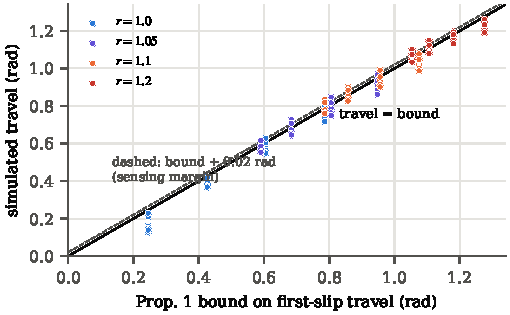
\includegraphics[width=\columnwidth]{fig_bound.pdf}
\caption{Proposition~\ref{prop:pivot} against simulation (V6). Each point is one release from a measured stuck grip. Points above the solid line exceed the bound; points above the dashed line exceed it by more than the sensing margin.}\label{fig:bound}
\end{figure}

\begin{table*}[t]\centering\footnotesize
\caption{Sliding test set (40 objects; learned methods: 5 seeds, 200 episodes per cell). Within: final error $\le$5\,mm and held. Over: travel past the target by more than 5\,mm. Probes: position measurements per episode. Shield $r_{\max}=1.2$.}\label{tab:slide}
\setlength{\tabcolsep}{3.2pt}
\begin{tabular}{llrrrrrrrrrrrr}
\toprule
 & & \multicolumn{3}{c}{$r=1.0$} & \multicolumn{3}{c}{$r=1.1$} & \multicolumn{3}{c}{$r=1.2$} & \multicolumn{3}{c}{$r=1.3$}\\
\cmidrule(lr){3-5}\cmidrule(lr){6-8}\cmidrule(lr){9-11}\cmidrule(lr){12-14}
ID & method & within & over & probes & within & over & probes & within & over & probes & within & over & probes\\
\midrule
B0 & model & 82 & 15 & 14.7 & 90 & 8 & 13.5 & 70 & 30 & 11.4 & 72 & 28 & 11.5\\
B0S & model + shield & 78 & \textbf{0} & 24.2 & 65 & 2 & 26.6 & 75 & 2 & 21.0 & 68 & 5 & 21.1\\
\midrule
B2 & residual & 90 & 8 & 9.3 & 90 & 10 & 8.2 & 89 & 11 & 7.4 & 86 & 13 & 7.9\\
B4 & residual, shield at test & 94 & 2 & 13.9 & 90 & 2 & 14.5 & 92 & \textbf{0} & 15.0 & 94 & \textbf{1} & 13.1\\
B5 & shield-trained residual & 98 & 2 & 12.1 & 98 & \textbf{1} & 11.9 & 96 & 2 & 11.4 & 96 & 2 & 10.8\\
\bottomrule
\end{tabular}
\end{table*}

\begin{table*}[t]\centering\footnotesize
\caption{Pivoting test set (40 objects; learned methods: 5 seeds, 200 episodes per cell). Within: final error $\le$0.05\,rad and held. Over: overshoot past the target by more than 0.05\,rad. Probes: angle measurements per pivot. Shield $r_{\max}=1.1$.}\label{tab:pivot}
\setlength{\tabcolsep}{3.2pt}
\begin{tabular}{llrrrrrrrrrrrr}
\toprule
 & & \multicolumn{3}{c}{$r=1.0$} & \multicolumn{3}{c}{$r=1.05$} & \multicolumn{3}{c}{$r=1.1$} & \multicolumn{3}{c}{$r=1.2$}\\
\cmidrule(lr){3-5}\cmidrule(lr){6-8}\cmidrule(lr){9-11}\cmidrule(lr){12-14}
ID & method & within & over & probes & within & over & probes & within & over & probes & within & over & probes\\
\midrule
B0 & model & 87.5 & 12.5 & 15.8 & 42.5 & 57.5 & 15.5 & 20 & 80 & 15.2 & 7.5 & 92.5 & 14.4\\
B1 & model + quasi-static guard & 87.5 & 12.5 & 16.2 & 42.5 & 57.5 & 15.7 & 20 & 80 & 15.4 & 7.5 & 92.5 & 14.6\\
B0S & model + shield & 85 & 7.5 & 19.8 & 42.5 & 47.5 & 19.1 & 22.5 & 70 & 18.0 & 7.5 & 80 & 16.9\\
B0Sd & model + shield (decline) & 7.5 & \textbf{0} & 13.2 & 12.5 & 2.5 & 12.6 & 17.5 & \textbf{2.5} & 11.6 & 7.5 & \textbf{30} & 11.1\\
\midrule
B2 & residual & 74 & 26 & 8.4 & 48.5 & 51.5 & 8.3 & 25.5 & 74.5 & 8.1 & 8 & 92 & 7.4\\
B3 & residual + quasi-static guard & 94 & 6 & 10.5 & 48 & 52 & 10.0 & 26.5 & 73.5 & 9.8 & 8 & 92 & 8.9\\
B4 & residual, shield at test & 88.5 & 3.5 & 18.3 & 47.5 & 45 & 18.0 & 26.5 & 65 & 16.7 & 9.5 & 82.5 & 15.5\\
B5 & shield-trained residual & 85 & 7 & 18.3 & 50.5 & 42 & 17.8 & 29 & 63 & 16.6 & 9.5 & 82.5 & 15.3\\
B5d & shield-trained (decline) & 10.5 & \textbf{0} & 11.6 & 12 & \textbf{1.5} & 11.3 & 21.5 & \textbf{2.5} & 10.2 & 9.5 & 32.5 & 9.9\\
\bottomrule
\end{tabular}
\end{table*}


\subsection{Q1: Does the shield keep the residual's savings?}
\emph{Sliding} (Table~\ref{tab:slide}). The unshielded residual B2 needs far fewer measurements than the model controller: \N{slide-1.2-B2-probes} against \N{slide-1.2-B0-probes} at $r=1.2$, and 3.5--5.3 fewer at every $r$. The shield-trained residual B5 keeps only part of this. It saves \N{slide-1.0-B5-dprobes} probes at $r=1.0$ (95\% CI \N{slide-1.0-B5-dprobeslo} to \N{slide-1.0-B5-dprobeshi}, Holm $p\N{slide-1.0-B5-pprobes}$) and \N{slide-1.1-B5-dprobes} at $r=1.1$ (not significant), and none at $r=1.2$ or 1.3. In sliding, then, the safety bought by the shield costs most of the residual's measurement saving. Two comparisons show where the cost goes. Shielding the unshielded residual only at test time (B4) needs 13.1--15.0 probes, against 10.8--12.1 for B5: a policy trained under the shield learns to work within it. Shielding the model controller (B0S) nearly doubles its probes, to 21--27. The shield shortens its holds, so the rod stops short and needs more pulses.

\emph{Pivoting} (Table~\ref{tab:pivot}). The unshielded residual again saves measurements: 7.0--7.4 fewer probes than the model at every $r$ (e.g.\ \N{pivot-1.1-B2-probes} against \N{pivot-1.1-B0-probes} at $r=1.1$). Under the shield this saving disappears entirely. B5 uses \emph{more} probes than B0, by \N{pivot-1.0-B5-dprobes} at $r=1.0$ (CI \N{pivot-1.0-B5-dprobeslo} to \N{pivot-1.0-B5-dprobeshi}) and by 1.0--2.3 at higher $r$. Training under the shield made no difference here: B4 and B5 are within 0.25 probes and 3.5 points of overshoot of each other at every $r$. Between 43 and 47\% of B5's steps were deferred to the model, so the policy rarely got to act. At $r=1$ the best trade-off belongs to the earlier quasi-static guard (B3: \N{pivot-1.0-B3-probes} probes, \N{pivot-1.0-B3-over}\% overshoot, \N{pivot-1.0-B3-within}\% within), but it stops helping as soon as $r>1$.

\subsection{Q2: Does the shield bound overshoot?}
\emph{Sliding.} The model controller overshoots \N{slide-1.0-B0-over}, \N{slide-1.1-B0-over}, \N{slide-1.2-B0-over} and \N{slide-1.3-B0-over}\% of episodes at $r=1.0$, 1.1, 1.2 and 1.3. The Coulomb prediction it uses for the hold underestimates the post-breakaway acceleration once $r>1$. The unshielded residual lowers this to 8--13\%. The shield-trained residual overshoots 1--2.5\% at every $r$, with 96--98\% of episodes ending within 5\,mm. Against B0, the reduction is \N{slide-1.2-B5-dovershoot} points at $r=1.2$ (CI \N{slide-1.2-B5-dovershootlo} to \N{slide-1.2-B5-dovershoothi}, Holm $p\N{slide-1.2-B5-povershoot}$) and \N{slide-1.3-B5-dovershoot} at $r=1.3$ (Holm $p\N{slide-1.3-B5-povershoot}$). At $r\le1.1$, where B0 overshoots less, the reduction is not significant after correction.

The certificate itself, that a certified pulse travels no further than its limit, failed on \N{slide-1.0-B5-viol}, \N{slide-1.1-B5-viol}, \N{slide-1.2-B5-viol} and \N{slide-1.3-B5-viol} of about 1\,900 certified B5 pulses per $r$ (0.15--0.35\%). Section~\ref{sec:q4} explains these failures.

\emph{Pivoting.} The model controller's overshoot grows steeply with $r$: \N{pivot-1.0-B0-over}, \N{pivot-1.05-B0-over}, \N{pivot-1.1-B0-over} and \N{pivot-1.2-B0-over}\%. The unshielded residual doubles it at $r=1$ (\N{pivot-1.0-B2-over}\%). With the defer fallback, the shield barely helps: B5 overshoots \N{pivot-1.0-B5-over}, \N{pivot-1.05-B5-over}, \N{pivot-1.1-B5-over} and \N{pivot-1.2-B5-over}\%, and no reduction against B0 survives Holm correction. Deferral hands control back to the model step precisely where the model overshoots. The decline fallback does stop overshoot within the assumed range: B5d overshoots \N{pivot-1.0-B5d-over}, \N{pivot-1.05-B5d-over} and \N{pivot-1.1-B5d-over}\% for $r\le r_{\max}$ (all $p<0.001$ against B0 for $r\ge1.05$). But it lands within the band on only \N{pivot-1.0-B5d-within}--\N{pivot-1.1-B5d-within}\% of episodes, because declined rods stop short, on average 0.35\,rad from the target. For $r\ge1.1$ no method ends within 0.05\,rad on more than 30\% of episodes (Fig.~\ref{fig:vsr}). Certified B5 steps violated their certificate on \N{pivot-1.0-B5-viol}, \N{pivot-1.05-B5-viol} and \N{pivot-1.1-B5-viol} of about 1\,600 for $r\le r_{\max}$ (at most 0.5\%).

\begin{figure*}[t]\centering
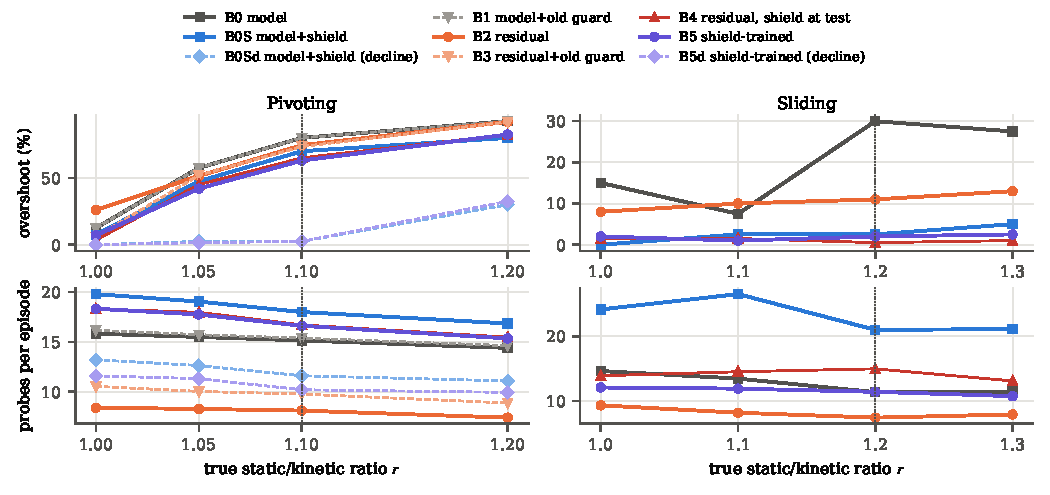
\includegraphics[width=\textwidth]{fig_vs_r.pdf}
\caption{Overshoot rate (top) and probes per episode (bottom) against the true static/kinetic ratio $r$, on the test sets. Dotted vertical line: the shield's assumed $r_{\max}$. In sliding the shield-trained residual (B5) stays near zero overshoot across $r$. In pivoting only the decline fallbacks (B0Sd, B5d) prevent overshoot, by stopping short.}\label{fig:vsr}
\end{figure*}

\subsection{Q3: How much of the task admits a certified action?}
\emph{Pivoting} is limited by Eq.~\eqref{eq:feas}. With $r_{\max}=1.1$, the equation predicts that 20 of the 40 test targets have no certified release from rest. The model controller with the decline fallback (B0Sd) declined at its very first step on exactly these 20 objects, both at $r=1.0$ and at $r=1.1$. A further 14 (at $r=1.0$) and 11 (at $r=1.1$) declined later, after 5--28 steps, once the rod had moved part of the way and the remaining arc could no longer be certified. Overall B0Sd declined on \N{pivot-1.0-B0Sd-declined}, \N{pivot-1.05-B0Sd-declined}, \N{pivot-1.1-B0Sd-declined} and \N{pivot-1.2-B0Sd-declined} of 40 objects. With the defer fallback, 53--61\% of steps were certified. The infeasible region is therefore not a corner case: for realistic friction ratios it covers most of the task.


\emph{Sliding} behaves as Proposition~\ref{prop:slide} predicts. Every shielded episode deferred exactly once, on its first pulse, while $F_{\rm stuck}$ was still unknown. No later pulse was infeasible, at any $r$ (B0S 160 of 160 episodes, B4 and B5 800 of 800 each).

\subsection{Q4: Why do violations and overshoots occur?}\label{sec:q4}
\emph{Attribution.} We replayed every test episode with a certificate violation and classified each violating step (an exploratory analysis, run after the pre-registered tests). For sliding, 10 of the 32 violating steps occurred at $r=1.3>r_{\max}$, where no guarantee applies. One followed a recorded stuck grip that was below the true arrest requirement: the rod had slipped by less than the 2.5\,mm motion threshold. The remaining 21 occurred with every assumption of Proposition~\ref{prop:slide} satisfied. All 21 were on three objects, all heavy ($m=0.178$--$0.192$\,kg). Direct probes on these objects found simulated travel up to 1.8 times the bound for short pulses released close to the stuck grip, where the bound is only a few millimetres. On light objects, travel stayed below the bound. We attribute these to MuJoCo's regularised friction, which lets a heavily loaded contact creep \cite{mujocoissue}; this is a simulator effect and not a sensing error.

For pivoting, violations rise roughly tenfold when the assumption fails: at $r=1.2>r_{\max}$, \N{pivot-1.2-B5-viol} of \N{pivot-1.2-B5-cert} certified B5 steps (\N{pivot-1.2-B5-violpct}\%) violated the certificate, and decline-mode overshoot rose to \N{pivot-1.2-B5d-over}\%. At $r\le r_{\max}$ the violation rate is consistent with the model--simulator gap measured in V6.

\emph{Mismatch.} Fig.~\ref{fig:mismatch} shows what happens when $r_{\max}$ is wrong. In sliding, assuming $r_{\max}=1.0$ when the true $r$ is 1.1 or 1.2 raises B5's overshoot to \N{slide-mis-r1.1_rmax1.0-B5-over} and \N{slide-mis-r1.2_rmax1.0-B5-over}\% and its violation rate to about 1\%. Its probes fall to \N{slide-mis-r1.2_rmax1.0-B5-probes}, the level of the unshielded residual. Assuming $r_{\max}=1.3$ keeps overshoot at \N{slide-mis-r1.2_rmax1.3-B5-over}--\N{slide-mis-r1.1_rmax1.3-B5-over}\% at a cost of \N{slide-mis-r1.2_rmax1.3-B5-probes} probes. The bound trades measurements for overshoot monotonically, and an underestimate degrades the shield gradually rather than abruptly. Pivoting behaves differently. With $r_{\max}=1.0$ every step is certifiable, but the certificates are wrong: \N{pivot-mis-r1.1_rmax1.0-B5-violpct}\% of B5's certified steps violated them at $r=1.1$. Yet B5's overshoot (\N{pivot-mis-r1.1_rmax1.0-B5-over}\%) is \emph{lower} than with $r_{\max}=1.2$ (\N{pivot-mis-r1.1_rmax1.2-B5-over}\%), where about 80\% of steps are deferred and no certificate is violated. A larger $r_{\max}$ hands more steps back to the model, which overshoots. With the defer fallback, a valid certificate on every certified step does not make the episode safe.

\begin{figure}[t]\centering
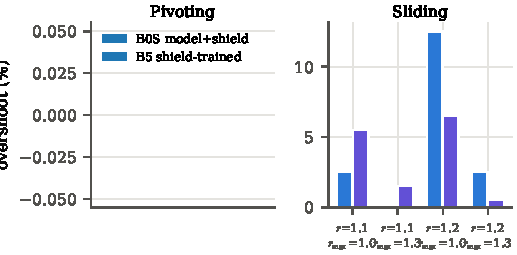
\includegraphics[width=\columnwidth]{fig_mismatch.pdf}
\caption{Overshoot of the shield-trained residual (B5, defer fallback) when the assumed $r_{\max}$ is wrong. Pivoting: $r_{\max}=1.0$, 1.1 (as trained) and 1.2. Sliding: 1.0, 1.2 (as trained) and 1.3. In sliding an underestimate raises overshoot and an overestimate lowers it. In pivoting the order reverses, because a larger $r_{\max}$ defers more steps to the overshooting model controller.}\label{fig:mismatch}
\end{figure}

\emph{Confirmation.} The confirmation sets, 40 fresh objects per task with $r$ drawn from the training range, were each run once after the test analysis had been committed. In sliding, B5 overshot \N{slide-conf-B5-over}\% of episodes against \N{slide-conf-B0-over}\% for B0 (Wilcoxon $p\N{slide-conf-B5-povershoot}$), ended within 5\,mm in \N{slide-conf-B5-within}\% against \N{slide-conf-B0-within}\%, and used \N{slide-conf-B5-probes} probes against \N{slide-conf-B0-probes} (difference not significant). The test-set conclusions replicate.
In pivoting ($r$ drawn from $[1.0,1.1]$), the confirmation set again showed no safety gain from the defer fallback: B5 overshot \N{pivot-conf-B5-over}\% against \N{pivot-conf-B0-over}\% for B0, while using \N{pivot-conf-B5-probes} probes against \N{pivot-conf-B0-probes} (Wilcoxon $p\N{pivot-conf-B5-pprobes}$). The decline fallback again removed overshoot (B0Sd \N{pivot-conf-B0Sd-over}\%) but declined on \N{pivot-conf-B0Sd-declined} of 40 objects and ended within the band on \N{pivot-conf-B0Sd-within}\%. No certified B5 step violated its certificate (\N{pivot-conf-B5-viol} of \N{pivot-conf-B5-cert}).


\section{Limitations}\label{sec:limits}
\textbf{Infeasible region.} The main limitation is physical rather than algorithmic. By \eqref{eq:feas}, no quasi-static release from rest can take the rod to a shallow target without passing it once $r$ exceeds $\varphi_{\lim}/\sin\varphi_{\lim}$. For $r=1.1$ this rules out every target shallower than about 0.75\,rad. In this region the shield can only defer, which reproduces the model controller's overshoot, or decline, which stops short. A fast slip-triggered re-clamp (a ``catch'') could reach these targets: in a separate probe, a 50\,ms detection-plus-clamp delay limited the first-slip jump to 0.03--0.07\,rad even at $r=1.5$. However, it needs slip detection far faster than our 10\,s current-based angle measurement, and we leave it to future work.

\textbf{Certified under a model, not under the world.} Proposition~\ref{prop:pivot} assumes a rigid rod, torsional capacity linear in grip, constant kinetic friction and no stored pad energy. In simulation the bound held on average, with simulated travel at 0.90--0.97 of the bound, but 24 of 128 direct test releases exceeded it by up to 0.048\,rad. We attribute this to soft-contact geometry, and it exceeds our 0.02\,rad sensing margin. On hardware, three effects could make the bound optimistic: soft-finger friction grows sub-linearly with load \cite{xydas1999}, so capacity falls faster than grip when grip is reduced; elastomer pads store torsional energy before breakaway; and static friction rises with dwell time \cite{dieterich1972}. A practical value of $r_{\max}$ should therefore be measured on the actual pad--object pair, at the hold times the controller uses, and taken from the upper tail of the measured ratios.

\textbf{Simulator.} MuJoCo has no true stick state \cite{mujocoissue}. We emulated static and kinetic friction by switching coefficients with hysteresis. The emulation reproduced the intended ratio (an emulated 1.2 measured 1.206) and an intrinsic ratio of 1.008, and first-slip travel was insensitive to the time step and switching thresholds. It is nonetheless a step-function Stribeck curve without rate-and-state effects \cite{canudas1995}. Kolbert et al.\ found that MuJoCo under-predicted a real pivot \cite{kolbert2016}, so absolute travel values should not be transferred to hardware.

\textbf{Learning and scope.} We used linear policies, evolution strategies, 1560 episodes per run and 5 seeds per method. Larger policies or other optimisers could change the comparison between shield-in-training and shield-at-test. Sensing during training was a noise model, not the motor-current pipeline. Lift-with-slip, the third task we originally planned, is not studied.


\section{Conclusion}
We asked when a learned correction should defer to a friction model at breakaway, and turned the answer into shields with closed-form certificates for pivoting and sliding. The answer depends on the task's physics more than on the learner. In sliding, a certified action almost always exists. A residual trained under the shield then keeps overshoot near zero across friction ratios, and degrades gradually when $r_{\max}$ is underestimated, although it gives up most of the unshielded residual's measurement saving. In pivoting, the stick--slip energy budget leaves no certified release for most shallow targets. There a shield cannot make a learned correction both efficient and safe: it can only choose between the model's overshoot and stopping short, and the feasibility condition $r<\varphi_{\lim}/\sin\varphi_{\lim}$ predicts in advance which targets force that choice. We see two next steps: a fast slip-triggered catch, which would enlarge the feasible region for pivoting, and measuring $r_{\max}$ on real pad--object pairs to test whether these certificates survive contact with hardware.


\section*{Acknowledgements and Disclosure}
Simulation code, analysis and drafting were carried out with the assistance of an AI model (Claude, Anthropic) under the author's direction. The author takes responsibility for the content. All results are from simulation.

\small
\bibliographystyle{unsrt}
\begin{thebibliography}{99}\setlength{\itemsep}{0pt}
\bibitem{johannink2019} T.~Johannink, S.~Bahl, A.~Nair, J.~Luo, A.~Kumar, M.~Loskyll, J.~A. Ojea, E.~Solowjow, and S.~Levine, ``Residual reinforcement learning for robot control,'' in \emph{Proc. IEEE ICRA}, 2019, arXiv:1812.03201.
\bibitem{silver2018} T.~Silver, K.~Allen, J.~Tenenbaum, and L.~Kaelbling, ``Residual policy learning,'' arXiv:1812.06298, 2018.
\bibitem{aidoo2026a} C.~Aidoo, ``Gravity pivoting from motor current: calibration-free angle estimation and the sensing budget it requires,'' engrXiv, doi:10.31224/8492, 2026.
\bibitem{aidoo2026b} C.~Aidoo, ``Residual learning on a physics pivoting controller: faster search, and where the quasi-static model breaks,'' engrXiv, doi:10.31224/8542, 2026.
\bibitem{alshiekh2018} M.~Alshiekh, R.~Bloem, R.~Ehlers, B.~K{\"o}nighofer, S.~Niekum, and U.~Topcu, ``Safe reinforcement learning via shielding,'' in \emph{Proc. AAAI}, 2018, arXiv:1708.08611.
\bibitem{ankile2024} L.~Ankile, A.~Simeonov, I.~Shenfeld, M.~Torne, and P.~Agrawal, ``From imitation to refinement -- residual RL for precise assembly,'' arXiv:2407.16677, 2024.
\bibitem{forcerft2026} Y.~Wang, C.~Zhang, X.~Su, J.~Ma, H.~Zhu, and X.~Li, ``ForceRFT: Refining VLA actions through force-guided residual reinforcement learning,'' arXiv:2609.22840, 2026.
\bibitem{chen2026priors} Y.~Chen, S.~Lu, E.~Colgate, and K.~Lynch, ``Robust in-hand manipulation via priors in reinforcement learning and mechanical design,'' arXiv:2607.12105, 2026.
\bibitem{cheng2019} R.~Cheng, G.~Orosz, R.~M. Murray, and J.~W. Burdick, ``End-to-end safe reinforcement learning through barrier functions for safety-critical continuous control tasks,'' in \emph{Proc. AAAI}, 2019, arXiv:1903.08792.
\bibitem{ames2019} A.~D. Ames, S.~Coogan, M.~Egerstedt, G.~Notomista, K.~Sreenath, and P.~Tabuada, ``Control barrier functions: theory and applications,'' in \emph{Proc. ECC}, 2019, arXiv:1903.11199.
\bibitem{fisac2019} J.~F. Fisac, A.~K. Akametalu, M.~N. Zeilinger, S.~Kaynama, J.~Gillula, and C.~J. Tomlin, ``A general safety framework for learning-based control in uncertain robotic systems,'' \emph{IEEE Trans. Autom. Control}, 2019, arXiv:1705.01292.
\bibitem{wabersich2021} K.~P. Wabersich and M.~N. Zeilinger, ``A predictive safety filter for learning-based control of constrained nonlinear dynamical systems,'' \emph{Automatica}, 2021, arXiv:1812.05506.
\bibitem{brunke2022} L.~Brunke, M.~Greeff, A.~W. Hall, Z.~Yuan, S.~Zhou, J.~Panerati, and A.~P. Schoellig, ``Safe learning in robotics: from learning-based control to safe reinforcement learning,'' \emph{Annu. Rev. Control Robot. Auton. Syst.}, 2022, arXiv:2108.06266.
\bibitem{kwon2026} M.~Kwon, T.~Ingebrand, U.~Topcu, and L.~Feng, ``Adaptive shielding for safe reinforcement learning under hidden-parameter dynamics shifts,'' arXiv:2506.11033, 2025.
\bibitem{ressafe2026} G.~Qu \emph{et al.}, ``ResSafe: learning safety filtering with residual reinforcement learning for humanoids,'' arXiv:2609.15988, 2026.
\bibitem{johansson2025} A.~Johansson, D.~Lindmark, V.~Wiberg, and M.~Servin, ``Safety filtering of robotic manipulation under environment uncertainty: a computational approach,'' arXiv:2509.12674, 2025.
\bibitem{shuto2026} Y.~Shuto and D.~V. Vargas, ``Sensorless damage-safe grasping,'' arXiv:2608.23983, 2026.
\bibitem{holladay2015} A.~Holladay, R.~Paolini, and M.~T. Mason, ``A general framework for open-loop pivoting,'' in \emph{Proc. IEEE ICRA}, 2015, pp.~3675--3681.
\bibitem{vina2016} F.~E. Vi{\~n}a B., Y.~Karayiannidis, C.~Smith, and D.~Kragic, ``Adaptive control for pivoting with visual and tactile feedback,'' in \emph{Proc. IEEE ICRA}, 2016, pp.~399--406.
\bibitem{toskov2022} J.~Toskov, R.~Newbury, M.~Mukadam, D.~Kuli{\'c}, and A.~Cosgun, ``In-hand gravitational pivoting using tactile sensing,'' in \emph{Proc. CoRL}, 2022, arXiv:2210.05068.
\bibitem{shi2017} J.~Shi, J.~Z. Woodruff, P.~B. Umbanhowar, and K.~M. Lynch, ``Dynamic in-hand sliding manipulation,'' \emph{IEEE Trans. Robot.}, 33(4):778--795, 2017.
\bibitem{chavandafle2015} N.~Chavan-Dafle and A.~Rodriguez, ``Prehensile pushing: in-hand manipulation with push-primitives,'' in \emph{Proc. IEEE/RSJ IROS}, 2015.
\bibitem{xydas1999} N.~Xydas and I.~Kao, ``Modeling of contact mechanics and friction limit surfaces for soft fingers in robotics, with experimental results,'' \emph{Int. J. Robot. Res.}, 18(9):941--950, 1999.
\bibitem{howe1996} R.~D. Howe and M.~R. Cutkosky, ``Practical force-motion models for sliding manipulation,'' \emph{Int. J. Robot. Res.}, 15(6):557--572, 1996.
\bibitem{kolbert2016} R.~Kolbert, N.~Chavan-Dafle, and A.~Rodriguez, ``Experimental validation of contact dynamics for in-hand manipulation,'' in \emph{Proc. ISER}, 2016, arXiv:1702.07252.
\bibitem{todorov2012} E.~Todorov, T.~Erez, and Y.~Tassa, ``MuJoCo: a physics engine for model-based control,'' in \emph{Proc. IEEE/RSJ IROS}, 2012, pp.~5026--5033.
\bibitem{mujocoissue} MuJoCo developers, ``Regularized friction never sticks,'' GitHub issue \#3328, google-deepmind/mujoco, 2026; and MuJoCo documentation, \emph{Computation: soft contacts}.
\bibitem{dieterich1972} J.~H. Dieterich, ``Time-dependent friction in rocks,'' \emph{J. Geophys. Res.}, 77(20):3690--3697, 1972.
\bibitem{canudas1995} C.~Canudas de Wit, H.~Olsson, K.~J. {\AA}str{\"o}m, and P.~Lischinsky, ``A new model for control of systems with friction,'' \emph{IEEE Trans. Autom. Control}, 40(3):419--425, 1995.
\end{thebibliography}

\end{document}
